
\chapter{Theoretical Background}
\label{chap:theory}

...some introduction scentence depending on into chapter...

%The visualization pipeline developed in this project is supposed to process data that is produced by the scientific code Fleur \cite{fleur}.

Fleur computes the electronic structure in crystals using the Density Functional Theory approach (DFT), which is the state of the art method for this problem. The many-body Schrödinger equation, that can be used to describe electrons in solids, is almost impossible to solve directly, because the storage of the wavefunctions of each of the $N$ electrons in the system at each spatial coordinate exceeds the memory of any currently available computer for even quite small $N$. This motivates the DFT approach, that uses two fundamental theorems to reduce the computational complexity of the many-body problem significantly: The Hohenberg-Kohn theorem allows to use the electron density instead of the $N$-electron wavefunctions to uniquely characterize the ground state of a system. With the Kohn-Sham equations, the interacting Hamiltonian of the system can be replaced by non-interacting equations with an effective potential. This approach reduces the dimensionality of the problem from $N^3$ to $3$ and trades the interacting Hamiltonian for a set of non-interacting equations that have to be solved self-consistently. In general, the DFT approach is not just limited to computations of electrons in crystals, but is also for example used in chemistry to compute nonperiodic molecules.
% 
The output of a DFT calculation includes various physical quantities (for example the 3-dimensional spatial electron density, which is the central quantity in DFT calculations), but for this project we focus on two quantities that are easy to interpret, already reduced in dimensionality and frequently used in both experimental and theoretical physics.

The band structure $E(\vec{k})$ represents the eigenenergies of the eigenfunctions of the Hamiltonian for each crystal momentum $\vec{k}$. It is the dispersion relation of electrons in the crystal and relates allowed momenta and energies. In general, $E(\vec{k})$ is defined at any point inside the Brillouin zone, which is a special choice of the unit cell in the reciprocal lattice of the crystal. Both, the real-space lattice and the reciprocal lattice are shown for a face centered cubic (fcc) crystal in figure \ref{fcc}. For larger unit cells with fewer symmetries, the Brillouin zone can be much more complicated than in the shown example. In order to reduce the dimensionality of $E(\vec{k})$ with $k \in {\rm I\!R}^3$, the dispersion relation is only sampled along a discrete one-dimensional path between high symmetry points in the Brillouin zone. This path still contains most of the relevant physical features.

\begin{figure}[htb!]
    \centering
    \begin{subfigure}{.5\textwidth}
        \centering
        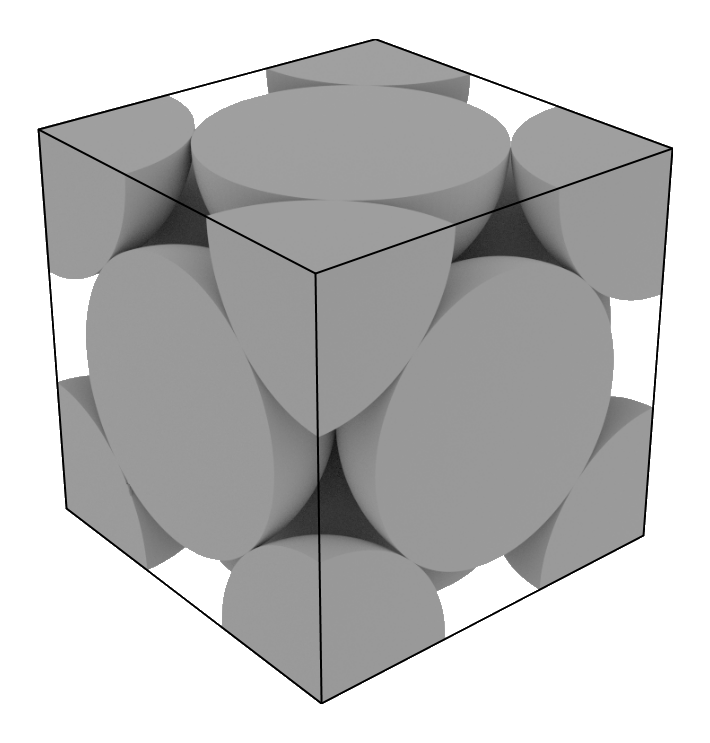
\includegraphics[width=0.5\linewidth]{christian/fcc_real.png}
        \caption{Lattice in real space}
        \label{fig:fcc_real}
    \end{subfigure}% %this '%' is needed for side-by-side figure!
    \begin{subfigure}{.5\textwidth}
        \centering
        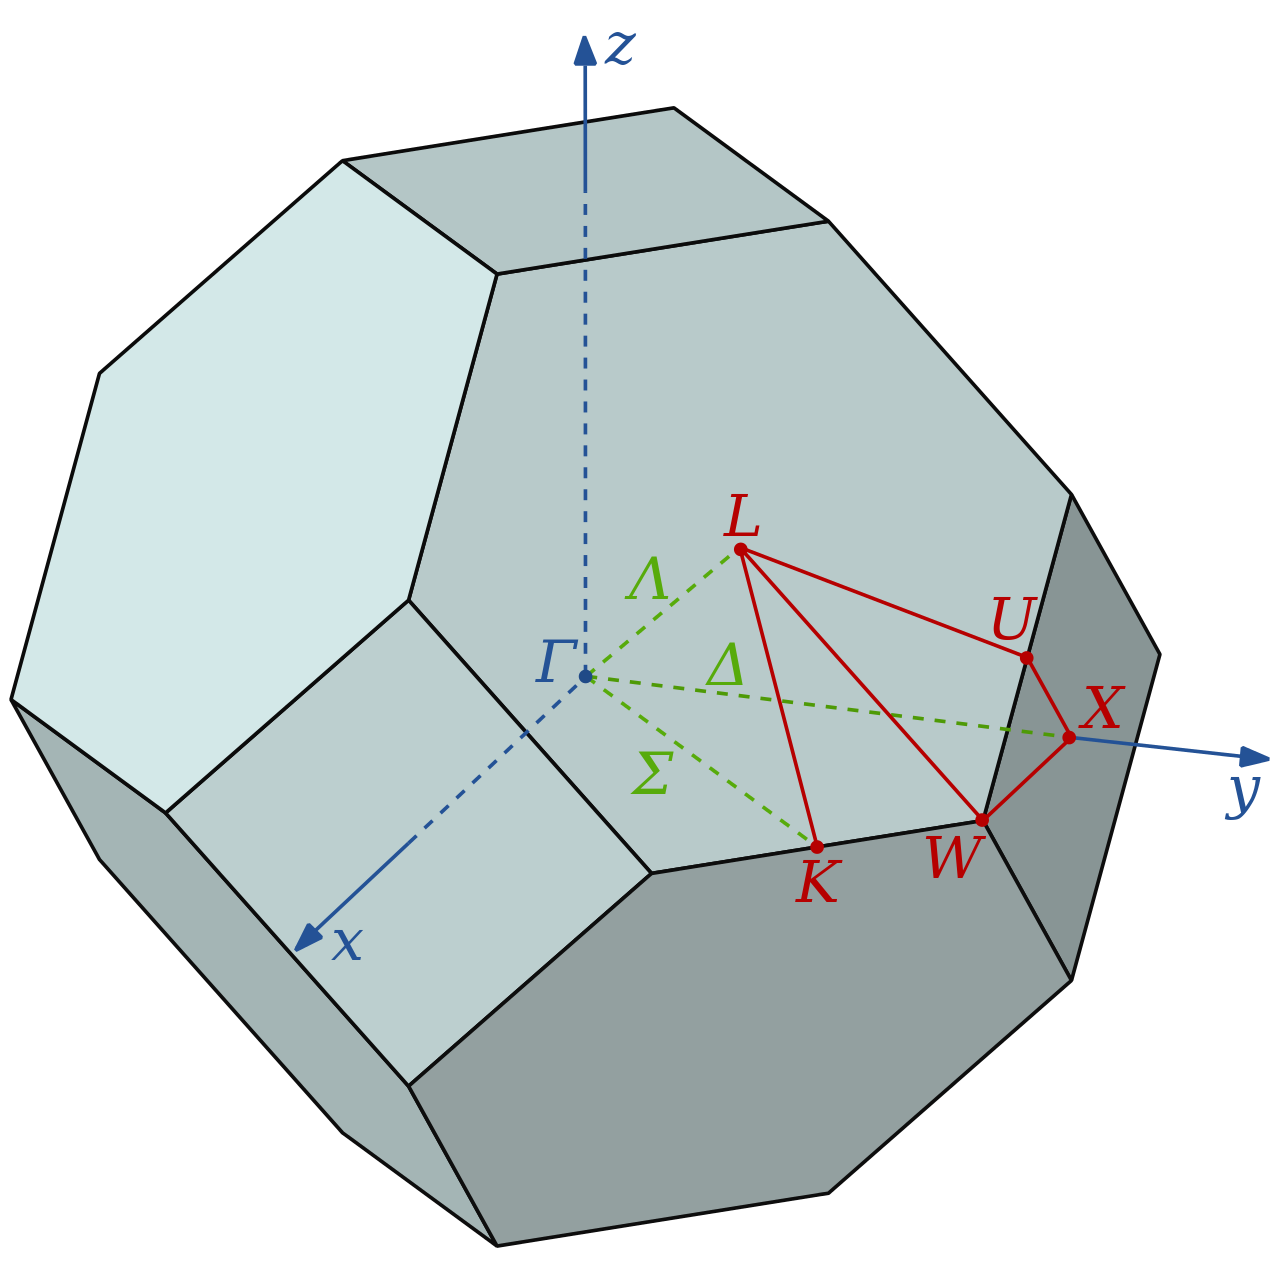
\includegraphics[width=0.5\linewidth]{christian/Brillouin_Zone_(1st,_FCC).png}
        \caption{Brillouin zone}
        \label{fig:fcc_billouin}
    \end{subfigure}
    \caption{Brillouin zone of a fcc lattice. The red curve in the reciprocal lattice represents a possible sampling path of $E(k)$ in the reciprocal lattice.}
    \label{fcc}
\end{figure}

The second central quantity in this project is the Density of States (DOS) $D(E)$, which describes the number of states per energy interval that is independent from the crystal momentum. In this sense, the DOS is also derived from $E(\vec{k})$, but instead of just selecting a subset, the $\vec{k}$ dependency is summed out. Both complementary quantities together are a common choice for comprehensive visualizations of electronic structure data while still capturing most of the important physics. 

For applications, it is useful to investigate where the contributions to $E(k)$ and $D(E)$ come from. Therefore, the data contains the weights of each basis function of the DFT calculation belonging to the individual atom groups and the orbitals. This means, spatial information about the system can be restored by considering only contributions from certain atom groups. (An atom group contains all atoms that are equivalent with respect to symmetries of the real space lattice.) On the other hand, the projection on the hydrogen orbitals s, p, d, f encode information about the shape of the wavefunction at each atom. These contributions are stored in the form of relative weights that can be summed to include contributions for multiple groups and orbitals. In case of distinct spins in the crystal, $E(k)$, $D(E)$ and the weights can be different for both spins and are therefore stored individually.



%%% Local Variables:
%%% mode: latex
%%% TeX-master: "../report"
%%% End:
